\chapter{Appendices}

\begin{figure}[htbp]
    \centering
    \begin{subfigure}[b]{0.5\textwidth}
        \centering
        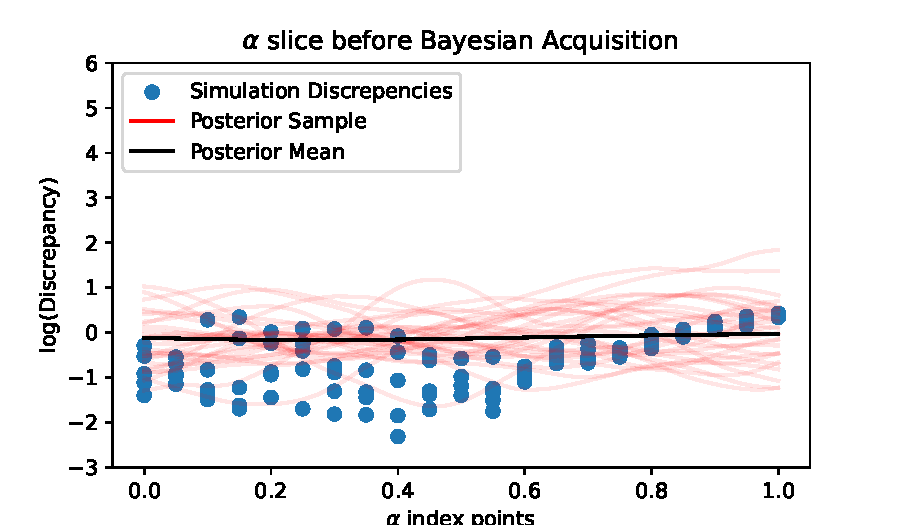
\includegraphics[width=\textwidth]{
            ../champagne_GP_images/initial_alpha_slice_log_discrep.pdf
        }
    \end{subfigure}%
    \hfill%
    \begin{subfigure}[b]{0.5\textwidth}
        \centering
        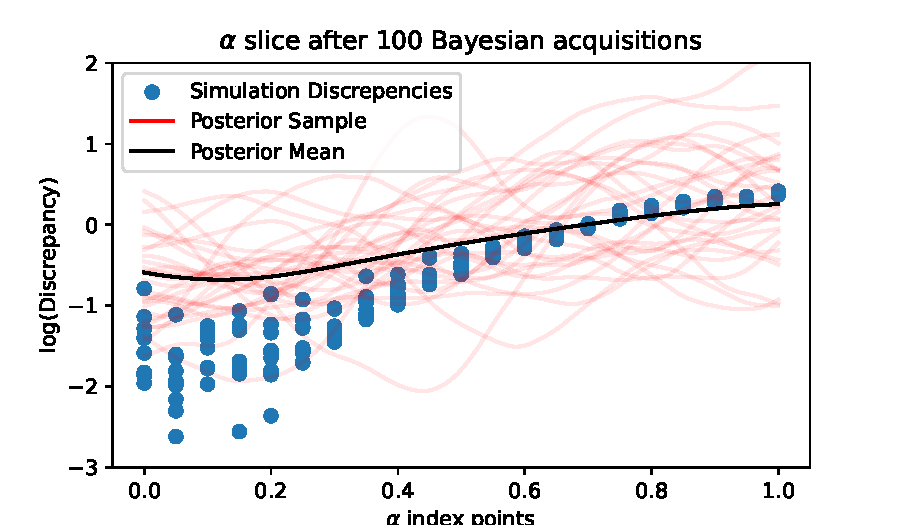
\includegraphics[width=\textwidth]{
            ../champagne_GP_images/alpha_slice_100_bolfi_updates_log_discrep.pdf
        }
    \end{subfigure}
    \hfill%
    \begin{subfigure}[b]{0.5\textwidth}
        \centering
        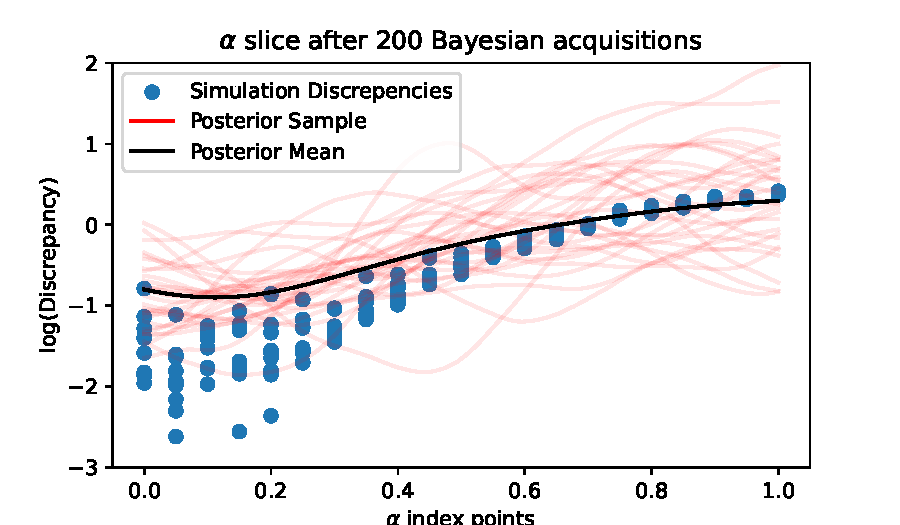
\includegraphics[width=\textwidth]{
            ../champagne_GP_images/alpha_slice_200_bolfi_updates_log_discrep.pdf
        }
    \end{subfigure}%
    \hfill%
    \begin{subfigure}[b]{0.5\textwidth}
        \centering
        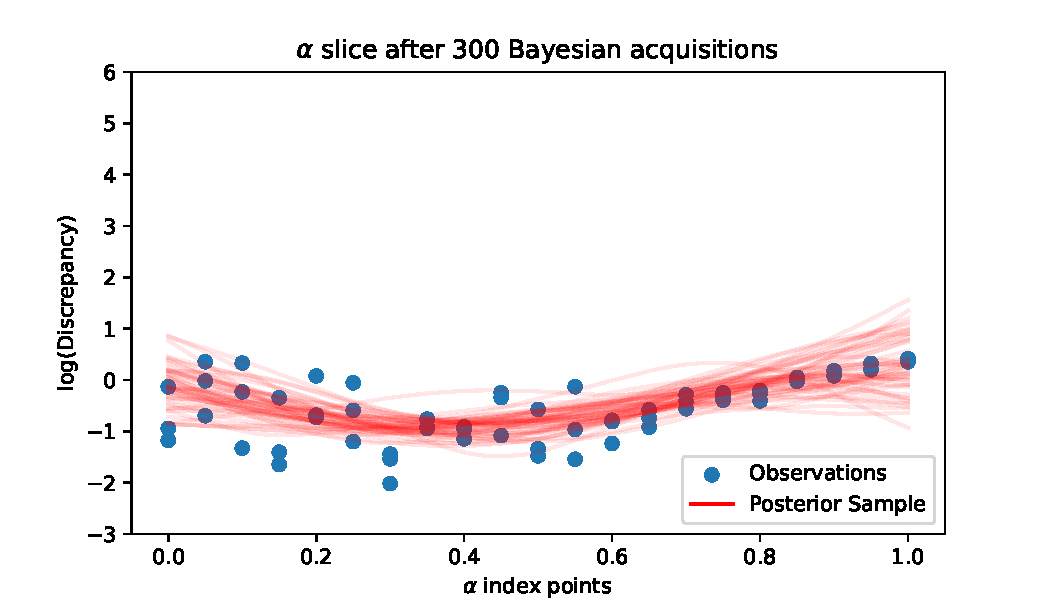
\includegraphics[width=\textwidth]{
            ../champagne_GP_images/alpha_slice_300_bolfi_updates_log_discrep.pdf
        }
    \end{subfigure}%
    \hfill%
    \begin{subfigure}[b]{0.5\textwidth}
        \centering
        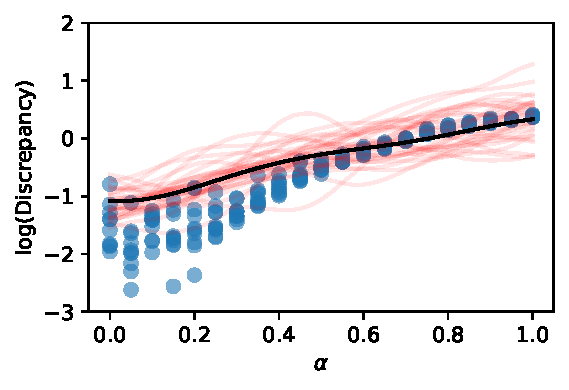
\includegraphics[width=\textwidth]{
            ../champagne_GP_images/alpha_slice_400_bolfi_updates_log_discrep.pdf
        }
    \end{subfigure}%
    \hfill%
    \begin{subfigure}[b]{0.5\textwidth}
        \centering
        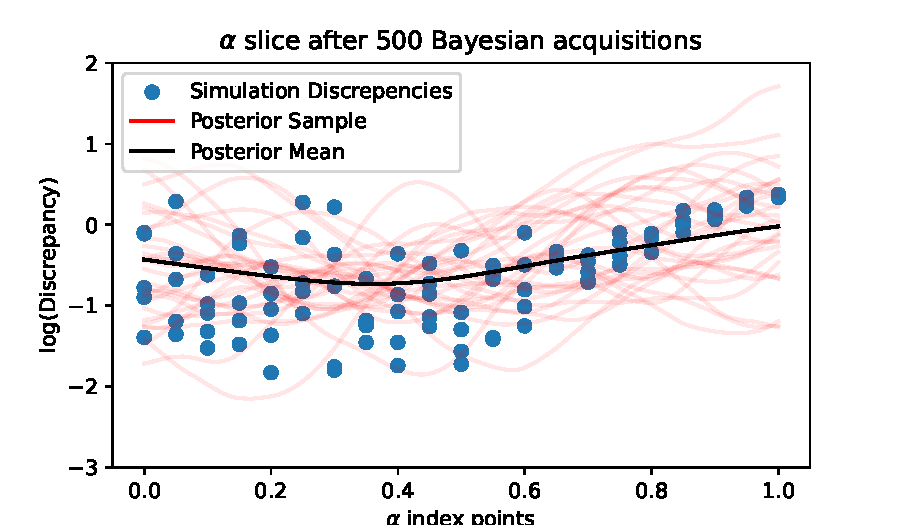
\includegraphics[width=\textwidth]{
            ../champagne_GP_images/alpha_slice_500_bolfi_updates_log_discrep.pdf
        }
    \end{subfigure}
    \caption{
        $d_\GP^{(t)}(\btheta)$ approximation of $\E(\ln\D(\btheta)),$ 
        for $t= 0$, $100$, $200$, $300$, $400$, and $500.$ Only $\alpha$ was 
        varied. All other parameters were fixed at the true values. Black line 
        is
        $\E(d^{(i)}(\btheta)).$
        Blue dots are realisations from $\ln\D(\btheta).$
    }
\end{figure}

\begin{figure}[htbp]
    \centering
    \begin{subfigure}[b]{0.5\textwidth}
        \centering
        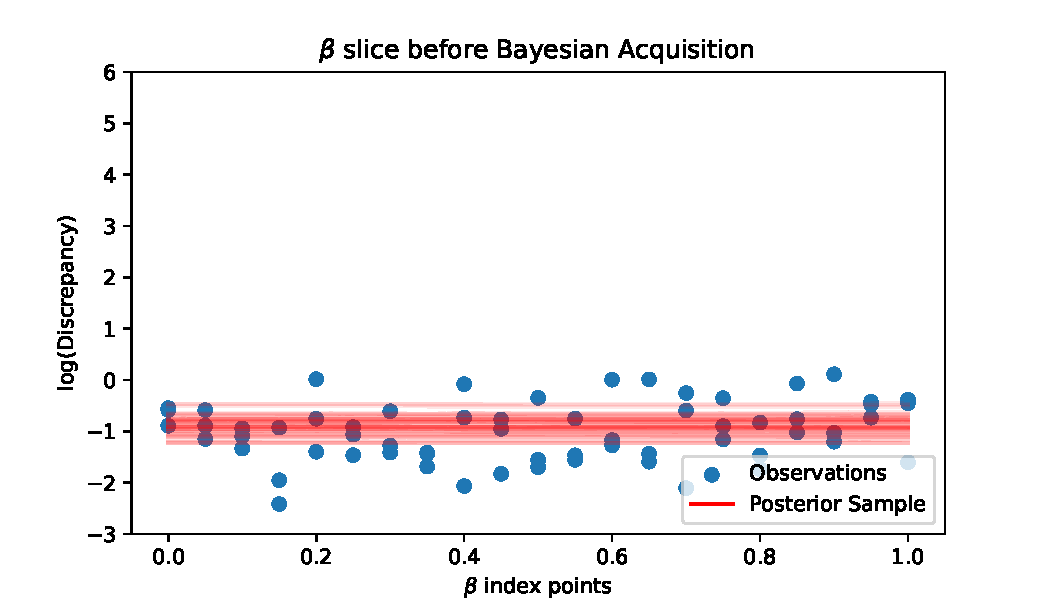
\includegraphics[width=\textwidth]{
            ../champagne_GP_images/initial_beta_slice_log_discrep.pdf
        }
    \end{subfigure}%
    \hfill%
    \begin{subfigure}[b]{0.5\textwidth}
        \centering
        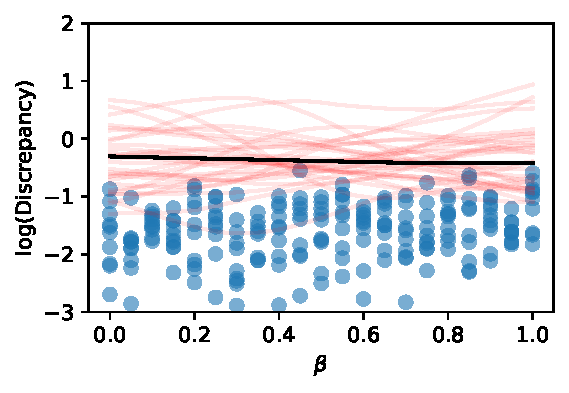
\includegraphics[width=\textwidth]{
            ../champagne_GP_images/beta_slice_100_bolfi_updates_log_discrep.pdf
        }
    \end{subfigure}
    \hfill%
    \begin{subfigure}[b]{0.5\textwidth}
        \centering
        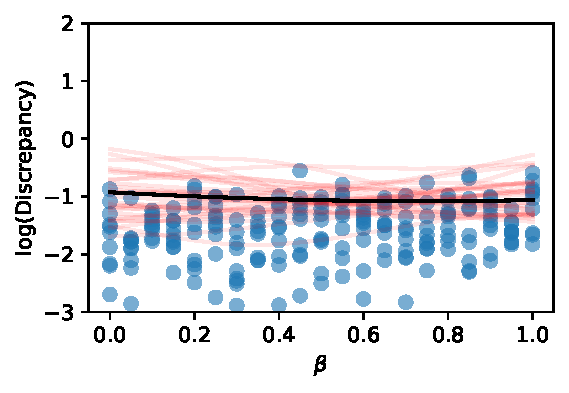
\includegraphics[width=\textwidth]{
            ../champagne_GP_images/beta_slice_200_bolfi_updates_log_discrep.pdf
        }
    \end{subfigure}%
    \hfill%
    \begin{subfigure}[b]{0.5\textwidth}
        \centering
        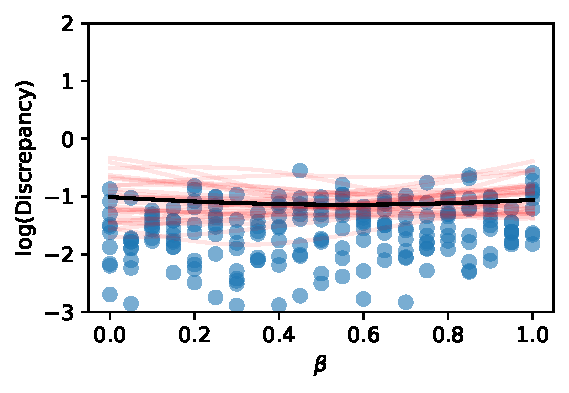
\includegraphics[width=\textwidth]{
            ../champagne_GP_images/beta_slice_300_bolfi_updates_log_discrep.pdf
        }
    \end{subfigure}%
    \hfill%
    \begin{subfigure}[b]{0.5\textwidth}
        \centering
        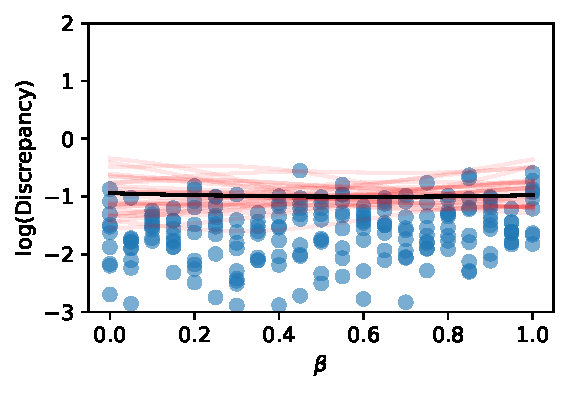
\includegraphics[width=\textwidth]{
            ../champagne_GP_images/beta_slice_400_bolfi_updates_log_discrep.pdf
        }
    \end{subfigure}%
    \hfill%
    \begin{subfigure}[b]{0.5\textwidth}
        \centering
        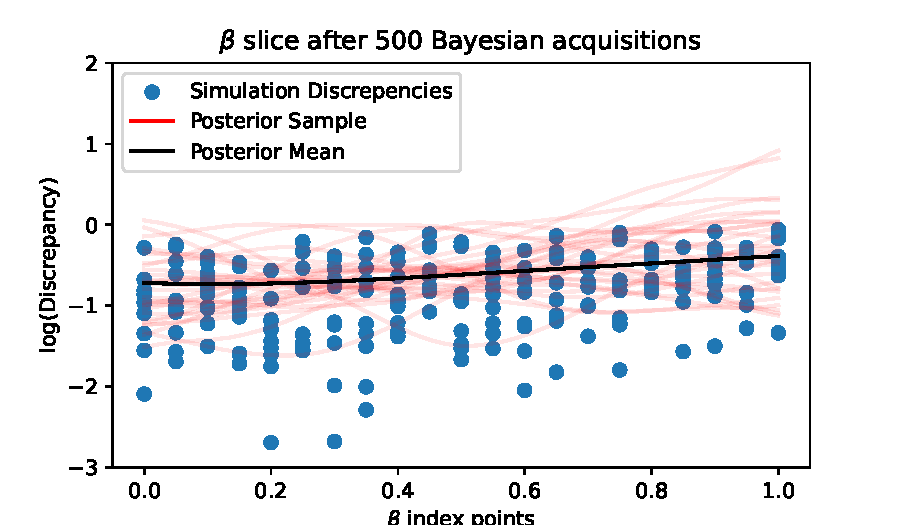
\includegraphics[width=\textwidth]{
            ../champagne_GP_images/beta_slice_500_bolfi_updates_log_discrep.pdf
        }
    \end{subfigure}
    \caption{
        $d_\GP^{(t)}(\btheta)$ approximation of $\E(\ln\D(\btheta)),$ 
        for $t= 0$, $100$, $200$, $300$, $400$, and $500.$ Only $\beta$ was 
        varied. All other parameters were fixed at the true values. Black line 
        is
        $\E(d^{(i)}(\btheta)).$
        Blue dots are realisations from $\ln\D(\btheta).$
    }
\end{figure}

\begin{figure}[htbp]
    \centering
    \begin{subfigure}[b]{0.5\textwidth}
        \centering
        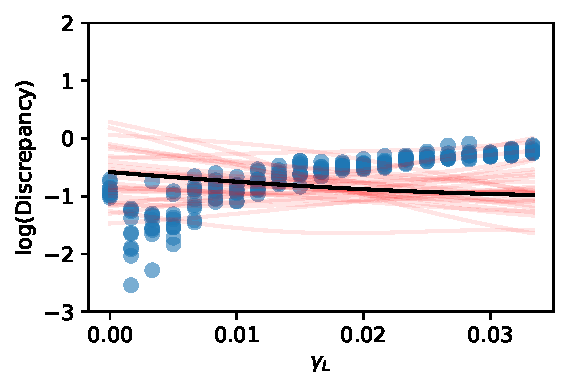
\includegraphics[width=\textwidth]{
            ../champagne_GP_images/initial_gamma_L_slice_log_discrep.pdf
        }
    \end{subfigure}%
    \hfill%
    \begin{subfigure}[b]{0.5\textwidth}
        \centering
        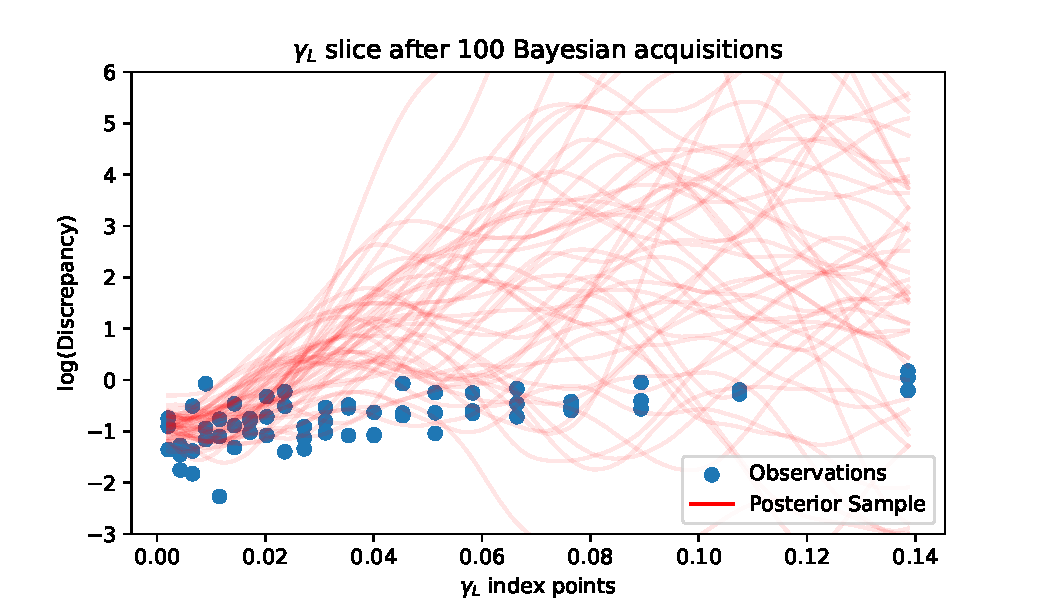
\includegraphics[width=\textwidth]{
            ../champagne_GP_images/gamma_L_slice_100_bolfi_updates_log_discrep.pdf
        }
    \end{subfigure}
    \hfill%
    \begin{subfigure}[b]{0.5\textwidth}
        \centering
        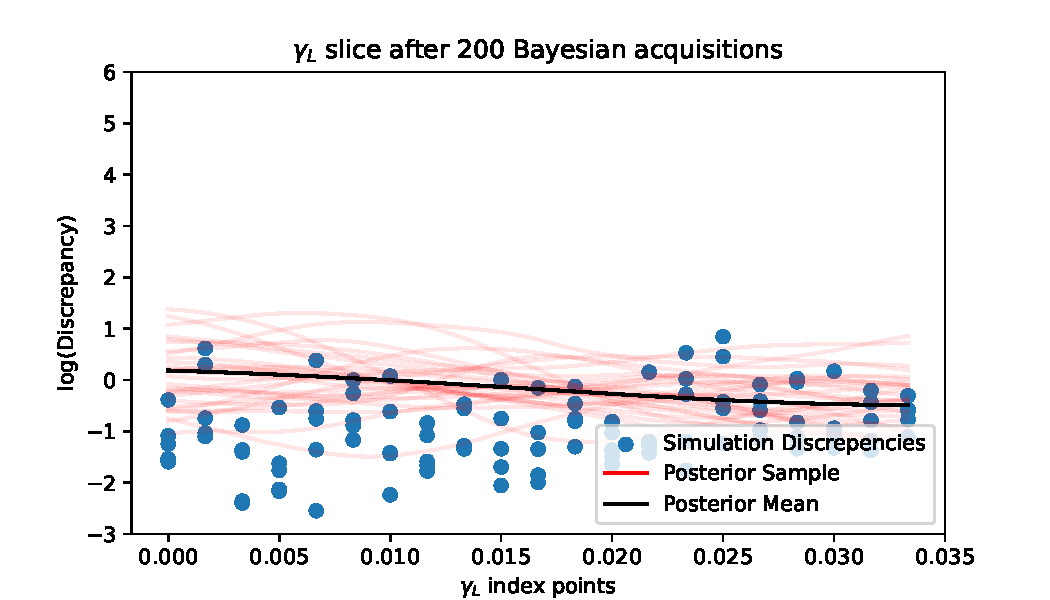
\includegraphics[width=\textwidth]{
            ../champagne_GP_images/gamma_L_slice_200_bolfi_updates_log_discrep.pdf
        }
    \end{subfigure}%
    \hfill%
    \begin{subfigure}[b]{0.5\textwidth}
        \centering
        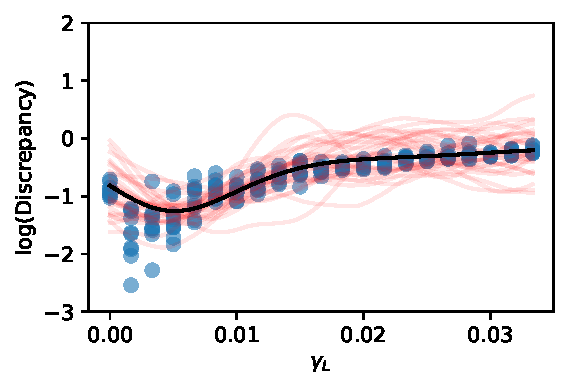
\includegraphics[width=\textwidth]{
            ../champagne_GP_images/gamma_L_slice_300_bolfi_updates_log_discrep.pdf
        }
    \end{subfigure}%
    \hfill%
    \begin{subfigure}[b]{0.5\textwidth}
        \centering
        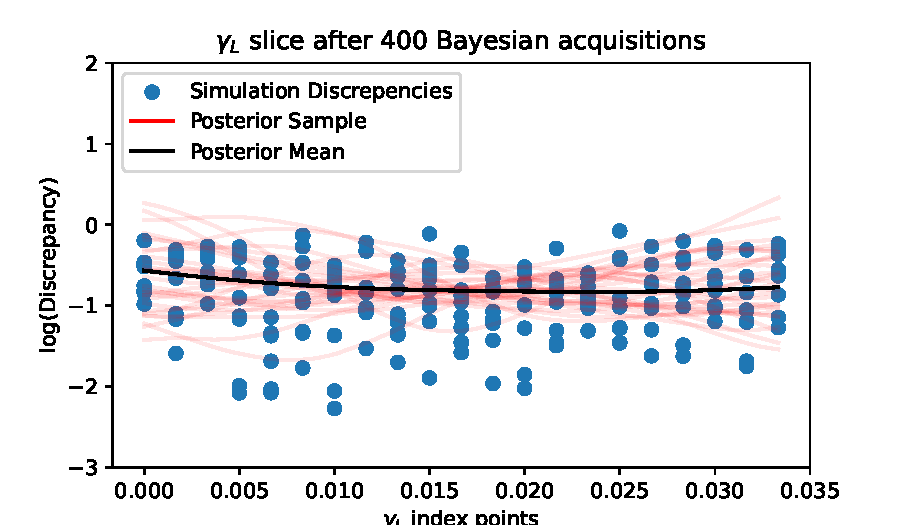
\includegraphics[width=\textwidth]{
            ../champagne_GP_images/gamma_L_slice_400_bolfi_updates_log_discrep.pdf
        }
    \end{subfigure}%
    \hfill%
    \begin{subfigure}[b]{0.5\textwidth}
        \centering
        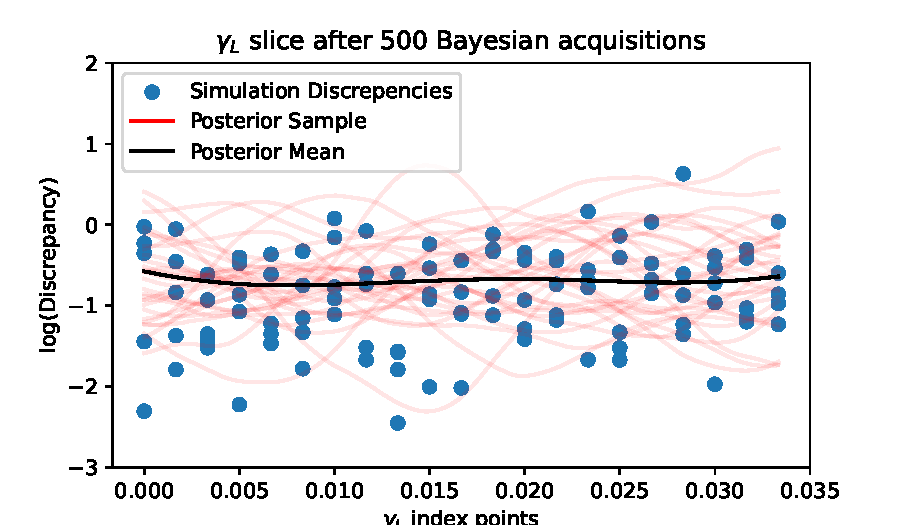
\includegraphics[width=\textwidth]{
            ../champagne_GP_images/gamma_L_slice_500_bolfi_updates_log_discrep.pdf
        }
    \end{subfigure}
    \caption{
        $d_\GP^{(t)}(\btheta)$ approximation of $\E(\ln\D(\btheta)),$ 
        for $t= 0$, $100$, $200$, $300$, $400$, and $500.$ Only $\gamma_L$ was 
        varied. All other parameters were fixed at the true values. Black line 
        is
        $\E(d^{(i)}(\btheta)).$
        Blue dots are realisations from $\ln\D(\btheta).$
    }
\end{figure}

\begin{figure}[htbp]
    \centering
    \begin{subfigure}[b]{0.5\textwidth}
        \centering
        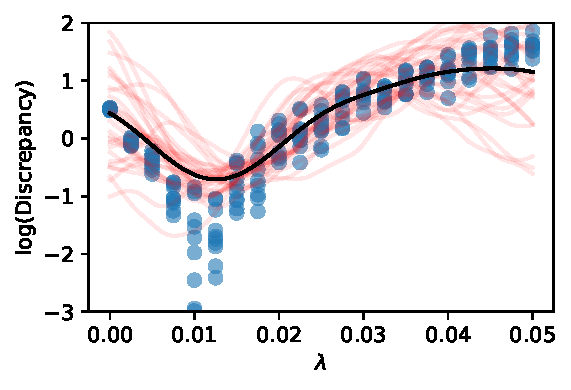
\includegraphics[width=\textwidth]{
            ../champagne_GP_images/initial_lambda_slice_log_discrep.pdf
        }
    \end{subfigure}%
    \hfill%
    \begin{subfigure}[b]{0.5\textwidth}
        \centering
        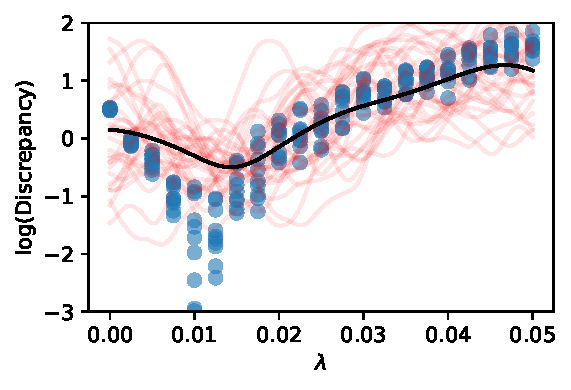
\includegraphics[width=\textwidth]{
            ../champagne_GP_images/lambda_slice_100_bolfi_updates_log_discrep.pdf
        }
    \end{subfigure}
    \hfill%
    \begin{subfigure}[b]{0.5\textwidth}
        \centering
        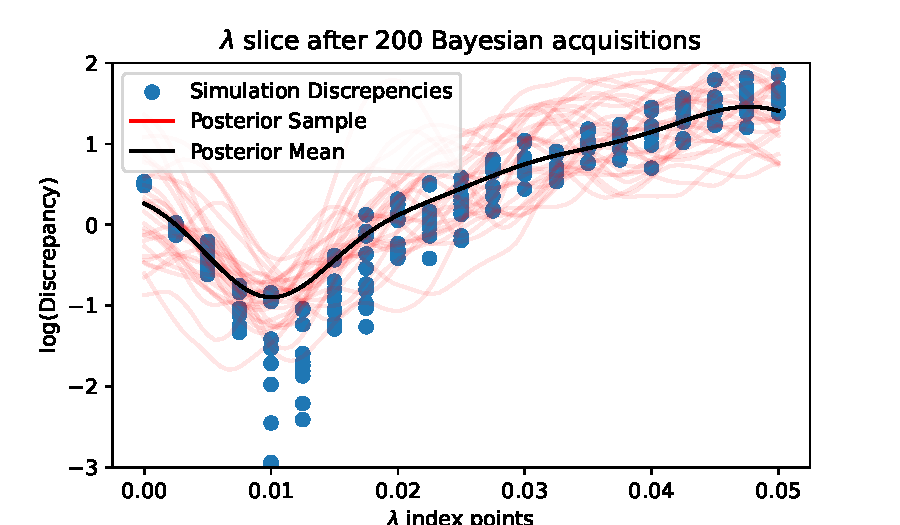
\includegraphics[width=\textwidth]{
            ../champagne_GP_images/lambda_slice_200_bolfi_updates_log_discrep.pdf
        }
    \end{subfigure}%
    \hfill%
    \begin{subfigure}[b]{0.5\textwidth}
        \centering
        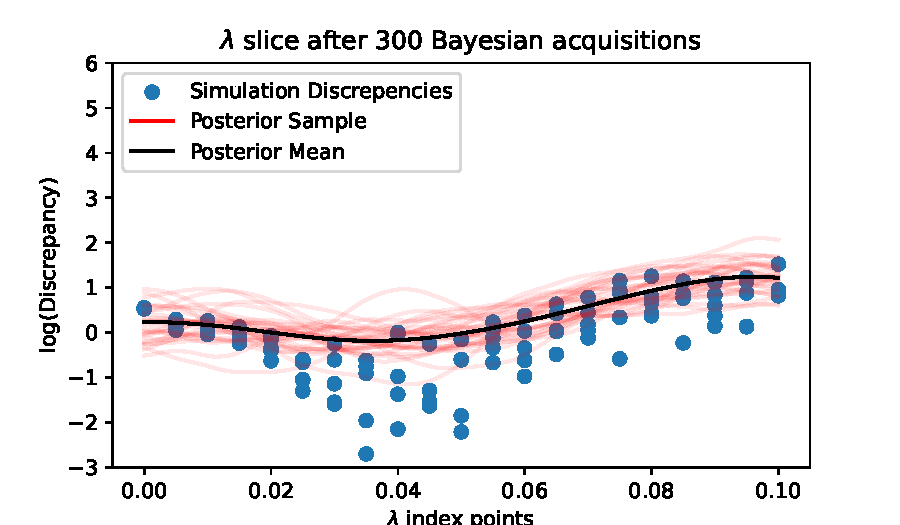
\includegraphics[width=\textwidth]{
            ../champagne_GP_images/lambda_slice_300_bolfi_updates_log_discrep.pdf
        }
    \end{subfigure}%
    \hfill%
    \begin{subfigure}[b]{0.5\textwidth}
        \centering
        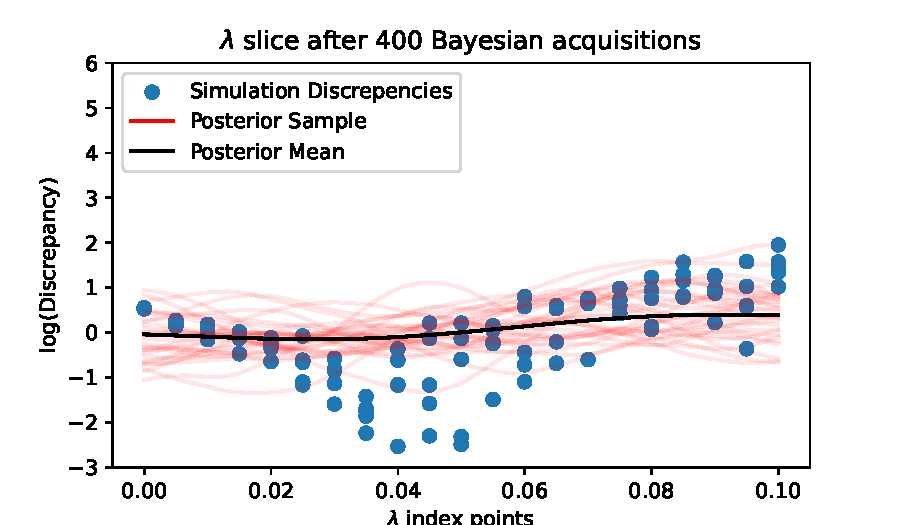
\includegraphics[width=\textwidth]{
            ../champagne_GP_images/lambda_slice_400_bolfi_updates_log_discrep.pdf
        }
    \end{subfigure}%
    \hfill%
    \begin{subfigure}[b]{0.5\textwidth}
        \centering
        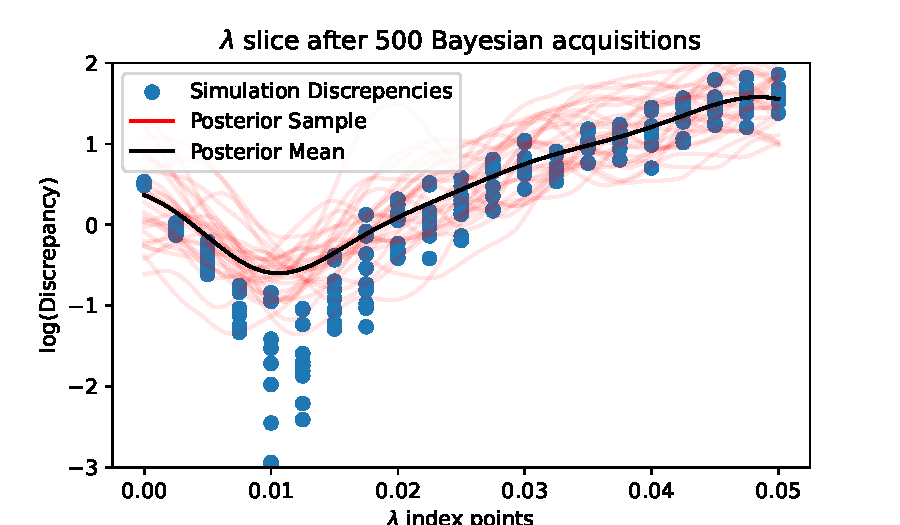
\includegraphics[width=\textwidth]{
            ../champagne_GP_images/lambda_slice_500_bolfi_updates_log_discrep.pdf
        }
    \end{subfigure}
    \caption{
        $d_\GP^{(t)}(\btheta)$ approximation of $\E(\ln\D(\btheta)),$ 
        for $t= 0$, $100$, $200$, $300$, $400$, and $500.$ Only $\lambda$ was 
        varied. All other parameters were fixed at the true values. Black line 
        is
        $\E(d^{(i)}(\btheta)).$
        Blue dots are realisations from $\ln\D(\btheta).$
    }
\end{figure}

\begin{figure}[htbp]
    \centering
    \begin{subfigure}[b]{0.5\textwidth}
        \centering
        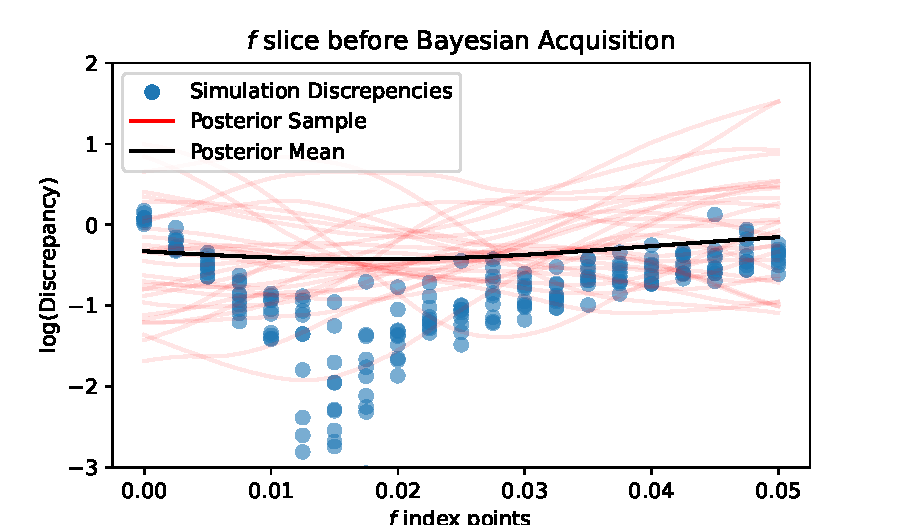
\includegraphics[width=\textwidth]{
            ../champagne_GP_images/initial_f_slice_log_discrep.pdf
        }
    \end{subfigure}%
    \hfill%
    \begin{subfigure}[b]{0.5\textwidth}
        \centering
        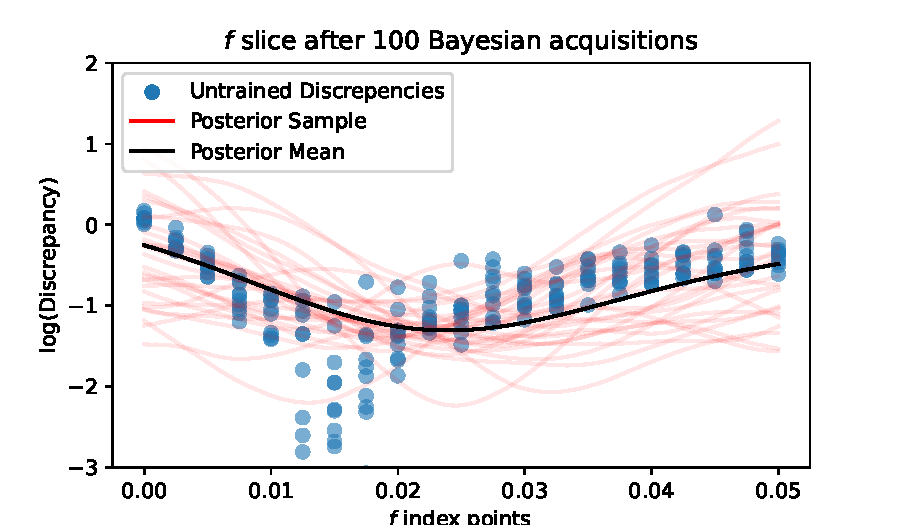
\includegraphics[width=\textwidth]{
            ../champagne_GP_images/f_slice_100_bolfi_updates_log_discrep.pdf
        }
    \end{subfigure}
    \hfill%
    \begin{subfigure}[b]{0.5\textwidth}
        \centering
        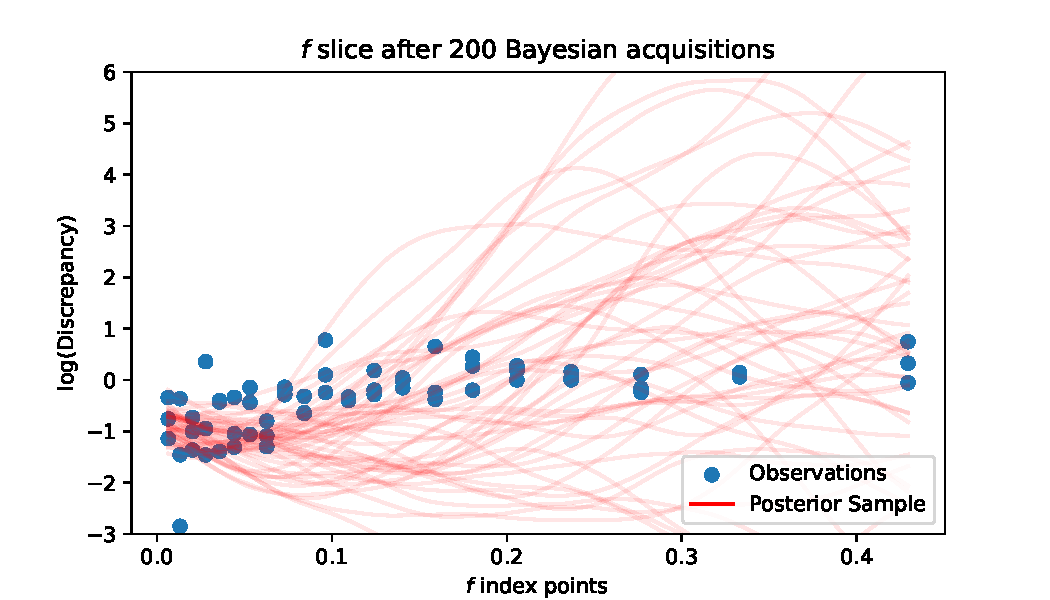
\includegraphics[width=\textwidth]{
            ../champagne_GP_images/f_slice_200_bolfi_updates_log_discrep.pdf
        }
    \end{subfigure}%
    \hfill%
    \begin{subfigure}[b]{0.5\textwidth}
        \centering
        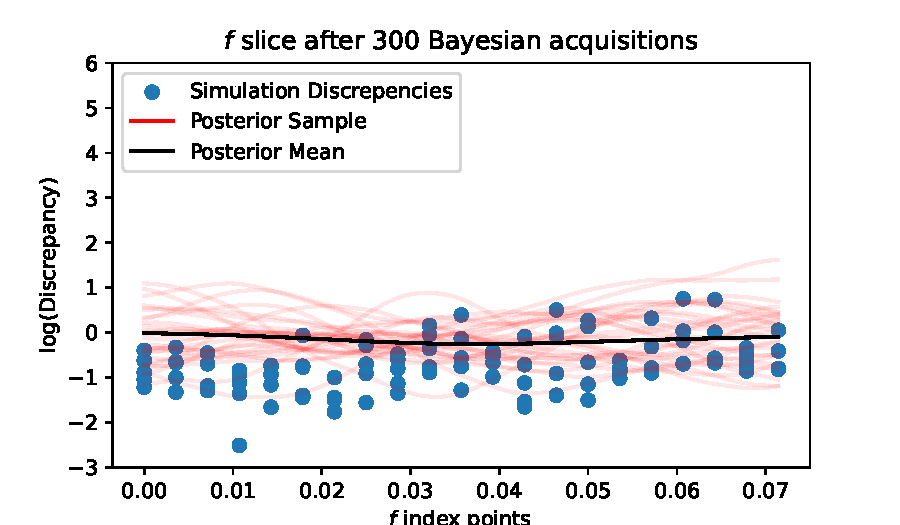
\includegraphics[width=\textwidth]{
            ../champagne_GP_images/f_slice_300_bolfi_updates_log_discrep.pdf
        }
    \end{subfigure}%
    \hfill%
    \begin{subfigure}[b]{0.5\textwidth}
        \centering
        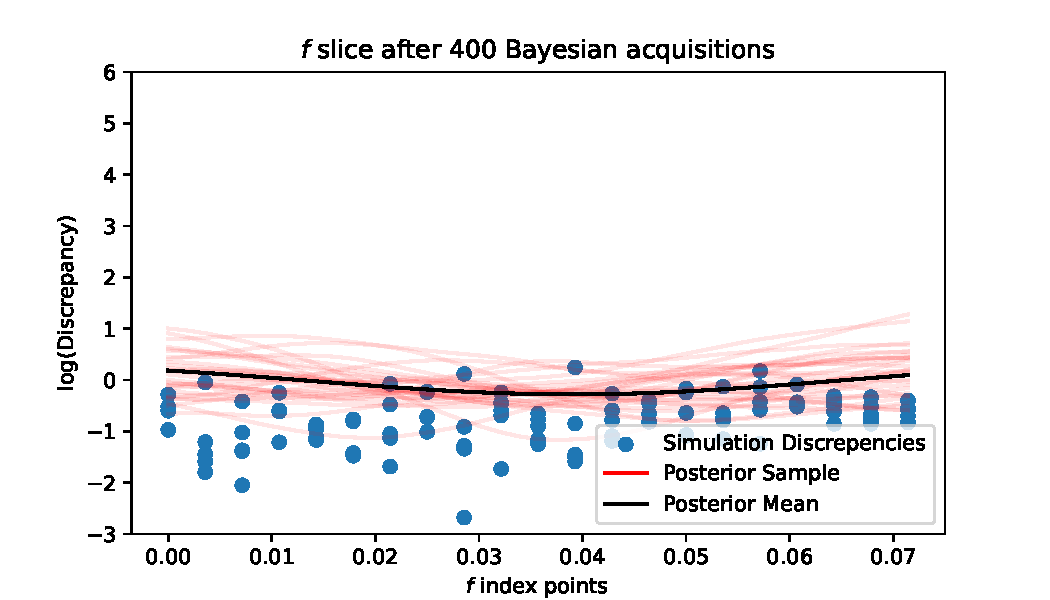
\includegraphics[width=\textwidth]{
            ../champagne_GP_images/f_slice_400_bolfi_updates_log_discrep.pdf
        }
    \end{subfigure}%
    \hfill%
    \begin{subfigure}[b]{0.5\textwidth}
        \centering
        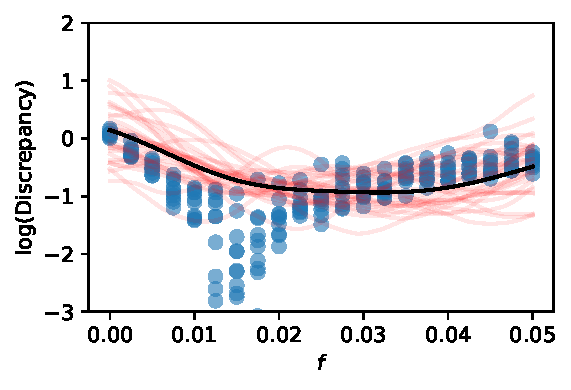
\includegraphics[width=\textwidth]{
            ../champagne_GP_images/f_slice_500_bolfi_updates_log_discrep.pdf
        }
    \end{subfigure}
    \caption{
        $d_\GP^{(t)}(\btheta)$ approximation of $\E(\ln\D(\btheta)),$ 
        for $t= 0$, $100$, $200$, $300$, $400$, and $500.$ Only $f$ was 
        varied. All other parameters were fixed at the true values. Black line 
        is
        $\E(d^{(i)}(\btheta)).$
        Blue dots are realisations from $\ln\D(\btheta).$
    }
\end{figure}

\begin{figure}[htbp]
    \centering
    \begin{subfigure}[b]{0.5\textwidth}
        \centering
        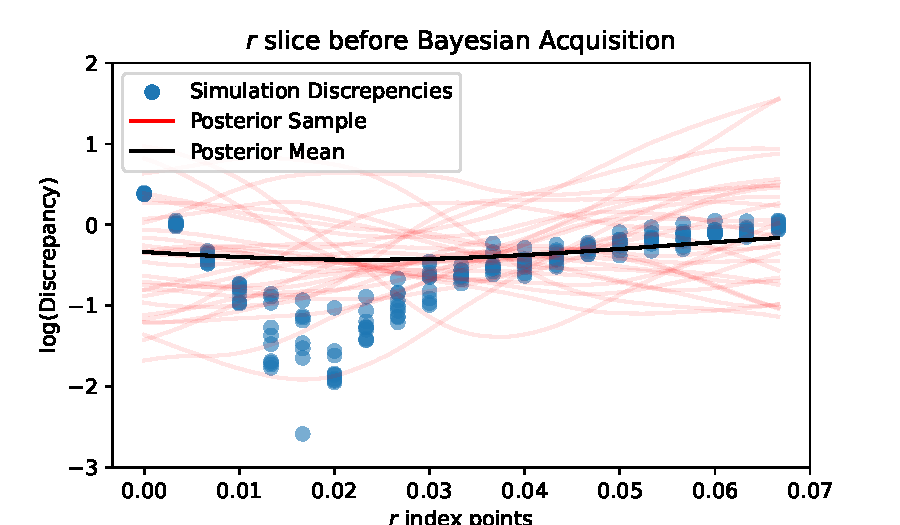
\includegraphics[width=\textwidth]{
            ../champagne_GP_images/initial_r_slice_log_discrep.pdf
        }
    \end{subfigure}%
    \hfill%
    \begin{subfigure}[b]{0.5\textwidth}
        \centering
        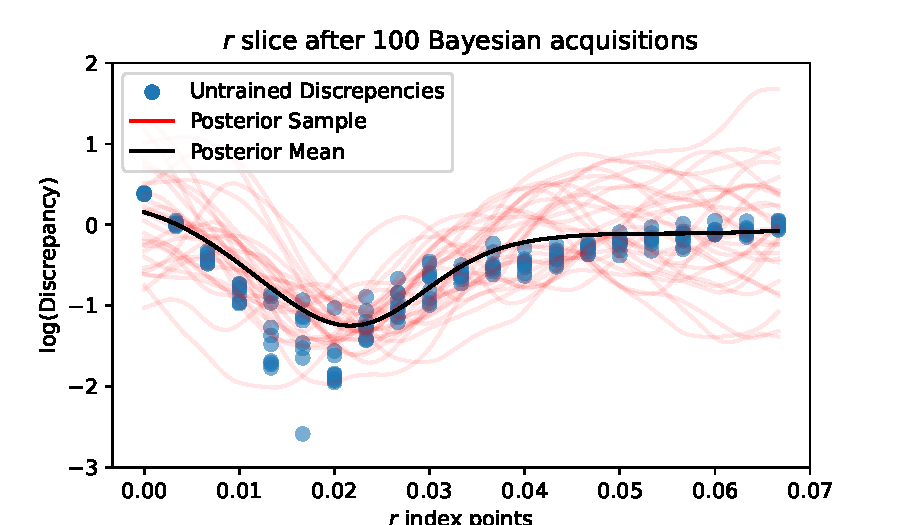
\includegraphics[width=\textwidth]{
            ../champagne_GP_images/r_slice_100_bolfi_updates_log_discrep.pdf
        }
    \end{subfigure}
    \hfill%
    \begin{subfigure}[b]{0.5\textwidth}
        \centering
        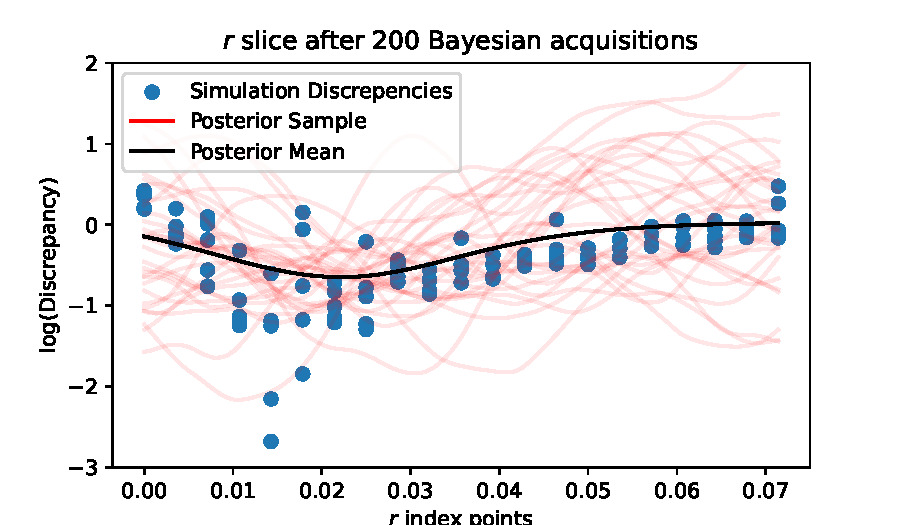
\includegraphics[width=\textwidth]{
            ../champagne_GP_images/r_slice_200_bolfi_updates_log_discrep.pdf
        }
    \end{subfigure}%
    \hfill%
    \begin{subfigure}[b]{0.5\textwidth}
        \centering
        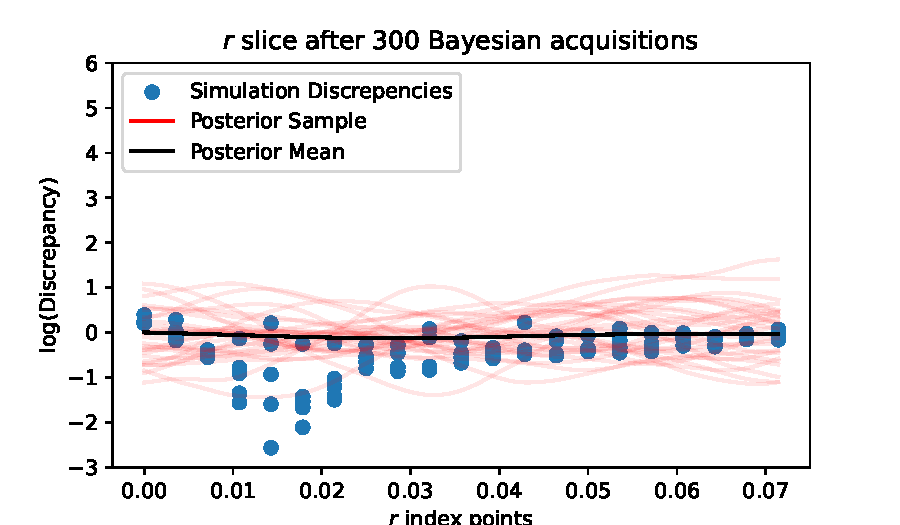
\includegraphics[width=\textwidth]{
            ../champagne_GP_images/r_slice_300_bolfi_updates_log_discrep.pdf
        }
    \end{subfigure}%
    \hfill%
    \begin{subfigure}[b]{0.5\textwidth}
        \centering
        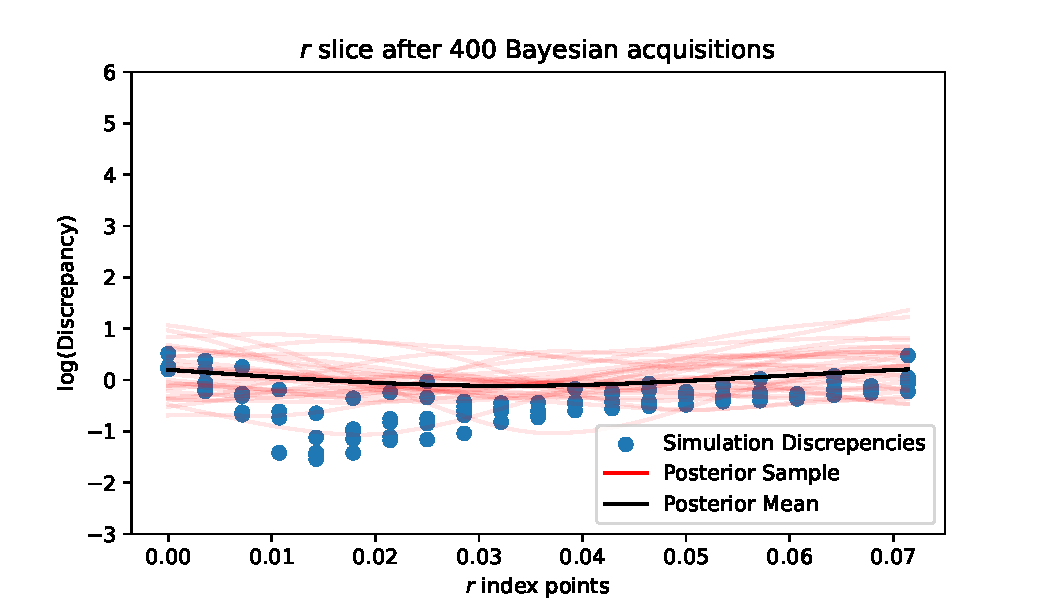
\includegraphics[width=\textwidth]{
            ../champagne_GP_images/r_slice_400_bolfi_updates_log_discrep.pdf
        }
    \end{subfigure}%
    \hfill%
    \begin{subfigure}[b]{0.5\textwidth}
        \centering
        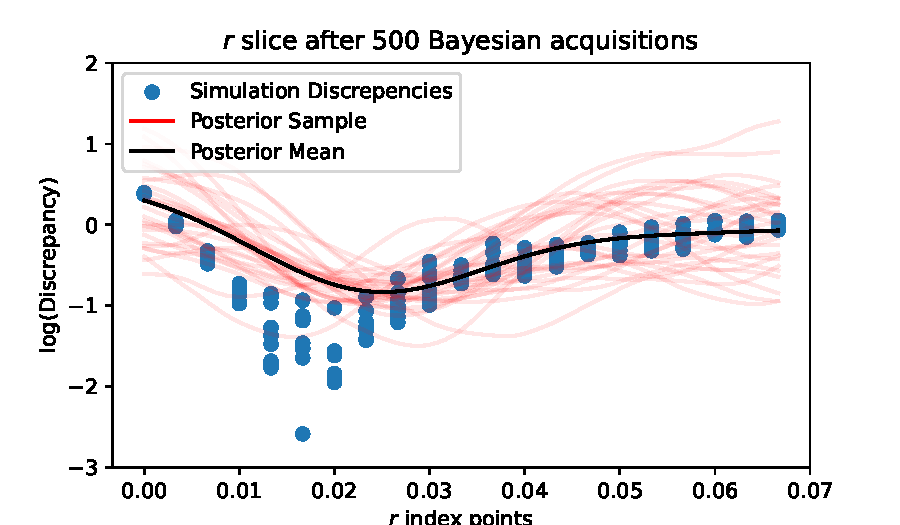
\includegraphics[width=\textwidth]{
            ../champagne_GP_images/r_slice_500_bolfi_updates_log_discrep.pdf
        }
    \end{subfigure}
    \caption{
        $d_\GP^{(t)}(\btheta)$ approximation of $\E(\ln\D(\btheta)),$ 
        for $t= 0$, $100$, $200$, $300$, $400$, and $500.$ Only $r$ was 
        varied. All other parameters were fixed at the true values. Black line 
        is
        $\E(d^{(i)}(\btheta)).$
        Blue dots are realisations from $\ln\D(\btheta).$
    }
\end{figure}